% **************************************************
% Document Class Definition
% **************************************************
\documentclass[%
    paper=A4,               % paper size --> A4 is default in Germany
    twoside=true,           % onesite or twoside printing
    openright,              % doublepage cleaning ends up right side
    parskip=half,           % spacing value / method for paragraphs
    chapterprefix=true,     % prefix for chapter marks
    11pt,                   % font size
    headings=normal,        % size of headings
    bibliography=totoc,     % include bib in toc
    listof=totoc,           % include listof entries in toc
    titlepage=on,           % own page for each title page
    captions=tableabove,    % display table captions above the float env
    chapterprefix=false,    % do not display a prefix for chapters
    appendixprefix=false,    % but display a prefix for appendix chapter
    draft=false,            % value for draft version
]{scrreprt}%


% **************************************************
% Setup YOUR thesis document in this file !
% **************************************************
% !TEX root = my-thesis.tex


% **************************************************
% Files' Character Encoding
% **************************************************
\PassOptionsToPackage{utf8}{inputenc}
\usepackage{inputenc}


% **************************************************
% Information and Commands for Reuse
% **************************************************
\newcommand{\thesisTitle}{Analyzing Bike Tracks Using Artificial Intelligence Algorithms}
\newcommand{\thesisName}{Nima Karimi}
\newcommand{\thesisSubject}{Documentation}
\newcommand{\thesisDate}{September 05, 2023}
\newcommand{\thesisVersion}{My First Draft}

% \newcommand{\thesisFirstReviewer}{Jane Doe}
% \newcommand{\thesisFirstReviewerUniversity}{\protect{Clean Thesis Style University}}
% \newcommand{\thesisFirstReviewerDepartment}{Department of Clean Thesis Style}

% \newcommand{\thesisSecondReviewer}{John Doe}
% \newcommand{\thesisSecondReviewerUniversity}{\protect{Clean Thesis Style University}}
% \newcommand{\thesisSecondReviewerDepartment}{Department of Clean Thesis Style}

\newcommand{\thesisFirstSupervisor}{Marta Disegna}
\newcommand{\thesisCoSupervisor}{Nicolò Biasetton}

\newcommand{\thesisUniversity}{\protect{University of Padova}}
\newcommand{\thesisUniversityDepartment}{Department of Management Engineering}
\newcommand{\thesisUniversityInstitute}{Institute for Clean Thesis Dev}
\newcommand{\thesisUniversityGroup}{Dipartimento di Tecnica e Gestione dei sistemi industriali}
\newcommand{\thesisUniversityCity}{Padova}
\newcommand{\thesisUniversityStreetAddress}{Street address}
\newcommand{\thesisUniversityPostalCode}{Postal Code}


% **************************************************
% Debug LaTeX Information
% **************************************************
%\listfiles


% **************************************************
% Load and Configure Packages
% **************************************************
\usepackage[english]{babel} % babel system, adjust the language of the content
\PassOptionsToPackage{% setup clean thesis style
    figuresep=colon,%
    hangfigurecaption=false,%
    hangsection=true,%
    hangsubsection=true,%
    sansserif=false,%
    configurelistings=true,%
    colorize=full,%
    colortheme=bluemagenta,%
    configurebiblatex=true,%
    bibsys=biber,%
    bibfile=bib-refs,%
    bibstyle=numeric,%
    bibsorting=none,%
}{cleanthesis}
\usepackage{cleanthesis}

\hypersetup{% setup the hyperref-package options
    pdftitle={\thesisTitle},    %   - title (PDF meta)
    pdfsubject={\thesisSubject},%   - subject (PDF meta)
    pdfauthor={\thesisName},    %   - author (PDF meta)
    plainpages=false,           %   -
    colorlinks=true,           %   - colorize links?
    linkcolor=BlueViolet,
    urlcolor=blue,
    citecolor=blue,
    % allcolors=blue,
    pdfborder={0 0 0},          %   -
    breaklinks=true,            %   - allow line break inside links
    bookmarksnumbered=true,     %
    bookmarksopen=true          %
}

% **************************************************
% Other Packages
% **************************************************
\usepackage{scrhack}



% **************************************************
% Listing Format
% **************************************************

\RequirePackage{listings}			% package for listings
% \lstset{%
%     backgroundcolor=\color{ctcolorgraylighter},
%     linewidth=\textwidth,
%     xleftmargin=10pt,
%     captionpos=b,
%     showspaces=false,
%     showstringspaces=false,
%     showtabs=false,
%     tabsize=2,
%     basicstyle=\footnotesize\ttfamily,
%     frame=leftline,
%     framerule=3pt,
%     framexleftmargin=4pt,
%     rulecolor=\color{ctcolorgraylight},
%     numbers=left,
%     numberstyle=\footnotesize\sffamily\color{ctcolorgray},
%     numbersep=15pt
% }
\lstset{
    language=Python,
    basicstyle=\ttfamily\small,
    backgroundcolor = \color{white},
    identifierstyle= \color{black},
    keywordstyle=\color{blue},
    commentstyle=\color{gray},
    stringstyle=\color{Green},
    numbers=left,
    numberstyle=\tiny\color{gray},
    rulecolor=\color{ctcolorgraylight},
    frame=single,
    framerule=3pt,
    breaklines=true
    linewidth=\textwidth,
    captionpos=b,
}




% **************************************************
% Document CONTENT
% **************************************************
\begin{document}

% uncomment the following command to fill up pages with
% whitespace instead of aligning the first and last lines
% of a page (see \raggedbottom vs. \flushbottom)
%\raggedbottom

% --------------------------
% rename document parts
% --------------------------

% > set short label names for floating environments figure and table
%\renewcaptionname{ngerman}{\figurename}{Abb.}
%\renewcaptionname{ngerman}{\tablename}{Tab.}
\renewcaptionname{english}{\figurename}{Fig.}
\renewcaptionname{english}{\tablename}{Tab.}

% > rename the title of the LOL, i.e. list of listings (default is "Listings")
\renewcommand*{\lstlistlistingname}{List of Listings}

% --------------------------
% Front matter
% --------------------------
\pagenumbering{roman}			% roman page numbing (invisible for empty page style)
\pagestyle{empty}				% no header or footers
% !TEX root = ../my-thesis.tex
%
% ------------------------------------  --> cover title page
% \begin{titlepage}
% 	\pdfbookmark[0]{Cover}{Cover}
% 	\flushright
% 	\hfill
% 	\vfill
% 	\vbox to0pt{\vbox to\textheight{\vfill \includegraphics[width=11.5cm]{resources/unipd-light} \vfill}\vss}
% 	{\LARGE\thesisTitle \par}
% 	\rule[5pt]{\textwidth}{.4pt} \par
% 	{\Large\thesisName}
% 	\vfill
% 	\textit{\large\thesisDate} \\
% 	Version: \thesisVersion
% \end{titlepage}


% ------------------------------------  --> main title page
\begin{titlepage}
	\pdfbookmark[0]{Titlepage}{Titlepage}
	% \tgherosfont
	\centering	
	
	\includegraphics[width=0.5\textwidth]{resources/unipd-800} \\[2mm]
	\vbox to0pt{\vbox to\textheight{\vfill \includegraphics[width=13cm]{resources/unipd-light} \vfill}\vss}
	
	\scshape{\huge{{\thesisUniversity}}} \\
	\line(1, 0){400} \\[2mm]


	\textsf{\thesisUniversityDepartment} \\
	% \textsf{\thesisUniversityInstitute} \\
	\textsf{\thesisUniversityGroup} \\

	\vfill
	% {\large \thesisSubject} \\[5mm]
	{\LARGE \color{ctcolortitle}\textbf{\thesisTitle} \\[10mm]}


	\begin{center}

	\vfill
	\begin{normalsize}
	\begin{flushleft}	  
	  \textit{Supervisors:} \hfill \textit{Master Candidate:}\\
		\vspace{1pt}

		%* names here
		Prof. \Large \thesisFirstSupervisor \hfill {\Large \thesisName} \\

		\vspace{20pt}

		\normalsize \textit{Co-Supervisors:} \\
		\vspace{1pt}
		\thesisCoSupervisor

		\vspace{30pt}
		\centering
		% \large{\textit{Academic Year} \\ 2023}
		Summer 2023
		% \thesisDate \\

	\end{flushleft}
	\end{normalsize}
	
	\end{center}
	\vspace*{\fill}
	\singlespacing
	\cleardoublepage


	\vfill
	% \begin{minipage}[t]{.27\textwidth}
	% 	\raggedleft
	% 	\textit{1. Reviewer}
	% \end{minipage}
	% \hspace*{15pt}
	% \begin{minipage}[t]{.65\textwidth}
	% 	{\Large \thesisFirstReviewer} \\
	%   	{\small \thesisFirstReviewerDepartment} \\[-1mm]
	% 	{\small \thesisFirstReviewerUniversity}
	% \end{minipage} \\[5mm]
	% \begin{minipage}[t]{.27\textwidth}
	% 	\raggedleft
	% 	\textit{2. Reviewer}
	% \end{minipage}
	% \hspace*{15pt}
	% \begin{minipage}[t]{.65\textwidth}
	% 	{\Large \thesisSecondReviewer} \\
	%   	{\small \thesisSecondReviewerDepartment} \\[-1mm]
	% 	{\small \thesisSecondReviewerUniversity}
	% \end{minipage} \\[10mm]
\end{titlepage}


% ------------------------------------  --> lower title back for single page layout
\hfill
\vfill
{
	\small
	\textbf{\thesisName} \\
	\textit{\thesisTitle} \\
	\thesisSubject, \thesisDate \\
	% Reviewers: \thesisFirstReviewer\ and \thesisSecondReviewer \\
	Supervisors: \thesisFirstSupervisor\ \\[1.5em]
	\textbf{\thesisUniversity} \\
	\textit{\thesisUniversityGroup} \\
	% \thesisUniversityInstitute \\
	\thesisUniversityDepartment \\
	% \thesisUniversityStreetAddress \\
	% \thesisUniversityPostalCode\ and 
	\thesisUniversityCity
}
		% INCLUDE: all titlepages
\cleardoublepage

\pagestyle{plain}				% display just page numbers
% !TEX root = ../my-thesis.tex
%
\pdfbookmark[0]{Abstract}{Abstract}
\addchap*{Abstract}
\label{sec:abstract}

This thesis presents a comprehensive study on developing a machine learning model to predict mobility patterns. The primary focus of this project is to utilize GPS data and assess the effectiveness of machine learning models in forecasting whether users use a lift on their way or not considering route characteristics. Additionally, the research aims to identify the key factors influencing mobility behavior and explore the potential application of machine learning models in personalized mobility prediction and sustainable transportation planning.

To achieve these objectives, a range of machine learning models will be evaluated for their accuracy and precision in forecasting mobility patterns. The research will investigate how different models perform in predicting mobility transportation. Moreover, an in-depth analysis will be conducted to identify the factors that significantly impact the accuracy of these models.

By examining the accuracy and precision of various machine learning models, this research will provide valuable insights into their effectiveness in mobility forecasting. Furthermore, it will uncover the factors that play a crucial role in influencing the accuracy of these models. The findings of this study will contribute to the advancement of machine learning applications in transportation planning and assist in developing personalized mobility prediction systems for sustainable transportation.

Keywords: machine learning, mobility patterns, accuracy, precision, personalized mobility prediction, sustainable transportation planning

\newpage

{\usekomafont{chapter}Riassunto}
\label{sec:abstract-it}

Questa tesi presenta uno studio completo sullo sviluppo di un modello di apprendimento automatico per prevedere i modelli di mobilità. L'obiettivo principale di questo progetto è utilizzare i dati GPS e valutare l'efficacia dei modelli di apprendimento automatico nel prevedere se gli utenti utilizzeranno un ascensore lungo il percorso o non considereranno le caratteristiche del percorso. Inoltre, la ricerca mira a identificare i fattori chiave che influenzano il comportamento di mobilità ed esplorare la potenziale applicazione dei modelli di apprendimento automatico nella previsione personalizzata della mobilità e nella pianificazione dei trasporti sostenibili.

Per raggiungere questi obiettivi, una serie di modelli di apprendimento automatico verranno valutati per la loro accuratezza e precisione nella previsione dei modelli di mobilità. La ricerca esaminerà le prestazioni dei diversi modelli nel prevedere la mobilità dei trasporti. Inoltre, verrà condotta un’analisi approfondita per identificare i fattori che incidono in modo significativo sull’accuratezza di questi modelli.

Esaminando l’accuratezza e la precisione di vari modelli di apprendimento automatico, questa ricerca fornirà preziose informazioni sulla loro efficacia nella previsione della mobilità. Inoltre, scoprirà i fattori che svolgono un ruolo cruciale nell’influenzare l’accuratezza di questi modelli. I risultati di questo studio contribuiranno al progresso delle applicazioni di apprendimento automatico nella pianificazione dei trasporti e aiuteranno nello sviluppo di sistemi di previsione della mobilità personalizzati per il trasporto sostenibile.

Parole chiave: machine learning, modelli di mobilità, accuratezza, precisione, previsione personalizzata della mobilità, pianificazione dei trasporti sostenibili

		% INCLUDE: the abstracts (english and german)
\cleardoublepage
%
% \input{content/acknowledgement} % INCLUDE: acknowledgement
\cleardoublepage
%
\currentpdfbookmark{\contentsname}{toc}
\setcounter{tocdepth}{2}		% define depth of toc
\tableofcontents				% display table of contents
\cleardoublepage

% --------------------------
% Body matter
% --------------------------
\pagenumbering{arabic}			% arabic page numbering
\setcounter{page}{1}			% set page counter
\pagestyle{scrheadings}			% header and footer style

%% Uncomment the following lines using the \part command
%% to add part sections
%\part{Example Part}
% !TEX root = ../my-thesis.tex
%
\chapter{Introduction}
\label{sec:intro}
With the rapid expansion of cities and the escalating worries regarding the sustainable use of our natural resources, the quest for achieving transportation systems that are not only efficient but also eco-friendly has garnered significant attention and become an urgent global challenge \cite{PRILLWITZ20111590}. 
Sustainable mobility, often referred to as sustainable transportation, aims to develop and implement strategies that promote the efficient movement of people and goods while minimizing negative environmental and social impacts \cite{su8010029, akerman2000european}. 
% Machine learning, a field of artificial intelligence, has emerged as a promising approach to addressing the complexities inherent in sustainable mobility by leveraging data-driven insights and advanced computational algorithms.

Furthermore, machine learning, a field of artificial intelligence, involves the development and application of computational models that can automatically learn and improve from data without explicit programming \cite{zhou2021machine}. 
By analyzing large and diverse datasets, machine learning algorithms can identify patterns, make predictions, and gain valuable insights that aid decision-making processes. In the context of sustainable mobility, machine learning can provide innovative solutions to optimize transportation systems \cite{wagner2022:urban-sm}, improve accessibility, and minimize environmental impact.

Mobility data has been leveraged to address inquiries such as estimating the demand of bus passengers based
on weather conditions utlizing a deep learning artificial neural network model as a regression model
~\cite{fontes2020deep}, using deep learning methods to discover the link between an individual's movement 
patterns and their personality traits~\cite{kim2018method}, examining large-scale mobile data to anticipate 
human trajectories, aiming to gain insights into human mobility patterns utilizing "DeepSpace" 
(An online deep learning framework)~\cite{ouyang2016deepspace}, how people travel between 
cities~\cite{reades2007cellular}, predicting the location of mobile users~\cite{anagnostopoulos2009predicting}.
\cite{toch2019analyzing} has conducted reviews of studies that examine location traces to extract insights about human mobility patterns.



Optimizing transportation systems through machine learning involves the application of data analytics to enhance operational efficiency, reduce congestion, and improve the overall performance of transportation networks. By processing large volumes of data collected from sources such as traffic sensors, GPS devices, and social media platforms, machine learning algorithms can generate real-time traffic predictions, optimize routing, and dynamically adapt transportation services \cite{anagnostopoulos2009predicting, dogra2022iot}. These advancements lead to improved travel experiences, reduced travel times, and more efficient allocation of resources.

Accessibility is a key aspect of sustainable mobility, aiming to ensure that transportation services are available and equitable for all individuals, regardless of their physical abilities, income levels, or geographic location. Machine learning algorithms can help address accessibility challenges by analyzing data on travel demand, demographics, and infrastructure characteristics \cite{de2021:ml:sustainable-transportation}. This enables the identification of underserved areas, optimization of transit routes, and the design of transportation services that cater to the needs of diverse populations \cite{cappelletti2022machine}.

Environmental sustainability is another critical dimension of sustainable mobility. Transportation accounts for a significant portion of global greenhouse gas emissions and is a major contributor to air pollution. Machine learning can play a crucial role in minimizing the environmental impact of transportation by developing predictive models that estimate emissions, optimize energy consumption, and facilitate the integration of clean and renewable energy sources \cite{castaneda2021:sustainable-transportation}. Additionally, machine learning techniques can aid in the design of eco-routing algorithms, which suggest the most environmentally friendly travel routes based on real-time data.

In summary, the combination of machine learning and sustainable mobility presents a promising framework to address the complex challenges faced by transportation systems. By harnessing the power of machine learning algorithms, transportation stakeholders can optimize operations, improve accessibility, and mitigate environmental impact. As the demand for sustainable and efficient mobility solutions continues to grow, machine learning can provide valuable insights and tools to shape the future of transportation, leading to more sustainable, accessible, and environmentally friendly mobility systems.


\section{Machine Learning}
\label{sec:intro:motivation}

Can computers learn like humans do from experience? Yes, through machine learning (ML).
It enhances system performance by using computational methods to learn 
from experience, mainly in the form of data. The key task in machine learning is developing
algorithms that build models from data. By inputting experience data into these algorithms,
we obtain models capable of predicting outcomes for new observations. In the context of
computer science, machine learning focuses on learning algorithms~\cite{zhou2021machine}.


~\cite{mitchell1997machine} provides a more formal definition: 
``A computer program is said to learn from experience E for some class of tasks T and performance measure P, 
if its performance at tasks in T, as measured by P, improves with experience E.``
The term "model" is broadly used to denote outcomes learned from data. In some literature 
(e.g.~\cite{hand2001principles}), "model" might mean a global outcome, while "pattern" signifies a local outcome.

The procedure of constructing models from data using machine learning algorithms is referred to as learning or training. The data employed during this phase is known as training data, where each sample serves as a training example, and the complete collection of training examples is the training set. The model derived from this process, representing the underlying data rules, is also termed a hypothesis, while the actual underlying rules are considered as facts or ground-truth. Thus, the fundamental goal of machine learning is to identify or approximate the ground-truth rules ~\cite{zhou2021machine}.

A wide range of machine-learning algorithms has been developed to address the diverse data and problem types in various machine-learning scenarios ~\cite{hastie2009elements, murphy2012machine}. These algorithms can be understood as exploring a vast space of potential programs, guided by training experience, to discover the most optimal performance. Variation among these algorithms arises from their methods of representing candidate programs, such as decision trees or mathematical functions, and their strategies for navigating this program space, including optimization techniques and evolutionary search methods~\cite{jordan2015machine}.

\subsection{Different Machine Learning algorithms}
Machine learning encompasses a wide range of learning types and algorithms. The major categories are supervised learning, unsupervised learning, semi-supervised learning, and reinforcement learning \cite{Alpaydin14}.

Supervised learning algorithms are trained on labeled data, which includes inputs and desired outputs. Common supervised tasks are classification, predicting categorical outputs like spam or not spam,
and regression, for instance predicting continuous values like price. Algorithms learn a mapping from inputs
to outputs by examining many examples. Supervised learning can achieve high 
predictive accuracy but relies on large labeled training sets which can be costly to obtain. 
Popular supervised algorithms include logistic regression, support vector machines, neural networks, decision trees, and random forests.

In contrast, unsupervised learning operates on unlabeled data, finding hidden patterns and intrinsic structure within it. Clustering algorithms are a key example, grouping data points that are similar. Other unsupervised techniques like dimensionality reduction and association rule mining also derive insights from the data itself without external labeling. As labeling is not required, unsupervised methods can more easily scale to new problem domains, but the models may not have clear accuracy measures.

In summary, machine learning employs various approaches to train models that can analyze data, recognize patterns, make predictions, or perform tasks. Supervised learning offers predictive accuracy but requires labeled data. Unsupervised learning can find hidden insights in any data without labeling but has less defined performance measures. Together these technologies enable machine learning systems to perform tasks not explicitly programmed.



\subsection{Overfitting}
\label{sec:overfit}


In supervised machine learning, an issue called overfitting arises, leading to poor generalization from observed data to new, unseen data. This results in a model performing well on the training set but poorly on the testing set. Overfitting occurs because the model becomes too specific to the training data and struggles with variations present in the testing data. Overfitted models tend to memorize noise and details of the training set rather than learning the underlying patterns~\cite{Ying_2019}.

Occam's Razor, or the principle of parsimony, advocates using models that contain only what's necessary for effective modeling. Overfitting occurs when models or procedures include more terms than needed, violating parsimony. Two types of overfitting are identified: using excessively flexible models and incorporating irrelevant components. Overfitting is undesirable due to resource wastage, potential prediction errors, worse decisions in feature selection, degraded predictions, and reduced portability of models. Portable models, adhering to Occam's Razor, are preferred for their broader applicability and reproducibility across locations~\cite{hawkins2004of,cook2016overfitting}.


\subsection{Spliting the dataset}

In both statistical and machine learning model development, a common practice is to divide the dataset into two parts: training and testing ~\cite{hastie2009elements}. The training set is utilized to estimate the model's unknown parameters, while the model's accuracy is assessed using the testing dataset. This division is essential to prevent overfitting, where a model becomes too tailored to the data, potentially leading to poor predictions in new situations. By reserving a subset of the data for testing, the model's performance can be evaluated before actual deployment, safeguarding against issues arising from overfitting.

The simplest and probably the most common strategy to split such a dataset is to randomly sample a fraction of the dataset. For example, 80\% of the rows of the dataset can be randomly chosen for training, and the remaining 20\% can be used for testing. Various strategies are showcased in ~\cite{roshan2022split} for efficiently and optimally dividing the dataset.

\subsection{Validation}
Furthermore, it's a frequent practice to reserve a segment of the training set for validation. This validation subset serves purposes such as refining model performance through hyper-parameter or regularization parameter selection (e.g. the number of hidden units—layers and layer widths—in a neural network~\cite{ripley2007pattern}). Validation datasets also can be used for regularization by early stopping (stopping training when the error on the validation data set increases, as this is a sign of over-fitting to the training data set)~\cite{Prechelt2012}.

To ensure greater result stability and maximize the use of valuable data for training, datasets can be repeatedly divided into multiple training and validation subsets. This practice, referred to as cross validation, is employed. Additionally, an independent test dataset held apart from cross-validation is typically utilized to validate the model's performance.~\cite{browne2000cv} provides an overview of various cross-validation techniques.

\section{Thesis Structure}
\label{sec:intro:structure}

\textbf{Chapter \ref{sec:data}} \\[0.2em]


\textbf{Chapter \ref{sec:model}} \\[0.2em]


\textbf{Chapter \ref{sec:results}} \\[0.2em]

   % INCLUDE: introduction
% !TEX root = ../my-thesis.tex
%
\chapter{Data Analysis}
\label{sec:data}

\cleanchapterquote{Information is the oil of the 21st century, and analytics is the combustion engine.}
{Peter Sondergaard}{(Founder of The Sondergaard Group, LLC.)}


This chapter discusses data analysis methodologies. Collaborating with \href{https://mowi.space/en}{Mowi Space}\footnote{\url{https://mowi.space/en}}, a platform tailored for mountain biking enthusiasts and winter sports enthusiasts, this collaboration has yielded a dynamic digital platform catering to outdoor sports. The Mowi website offers real-time data and interactive 3D maps for offline exploration. It delivers current trail conditions, weather updates, lift operations, and local events, ensuring informed and safe adventures. Notably, the Live Track feature allows real-time monitoring of family or friends during mountain activities, fostering connectivity and safety. This collaboration signifies a pivotal advancement in outdoor experience planning, merging technology with nature's allure.

As a result of getting some user's data going through various tracks,
it is possible to convert the GPS data into CSV files.

Fig. \ref{fig:track-gpx} is the example of one of the tracks plotted by 
\href{https://gpx.studio/}{GPX Studio}\footnote{\url{https://gpx.studio/}} and 
Fig. \ref{fig:track-csv} is plotted by the Python DataFrame which is a proof of accuracy of the DataFrame.

\begin{figure}[htb]
    \centering

    \begin{minipage}{\textwidth}
        \centering
        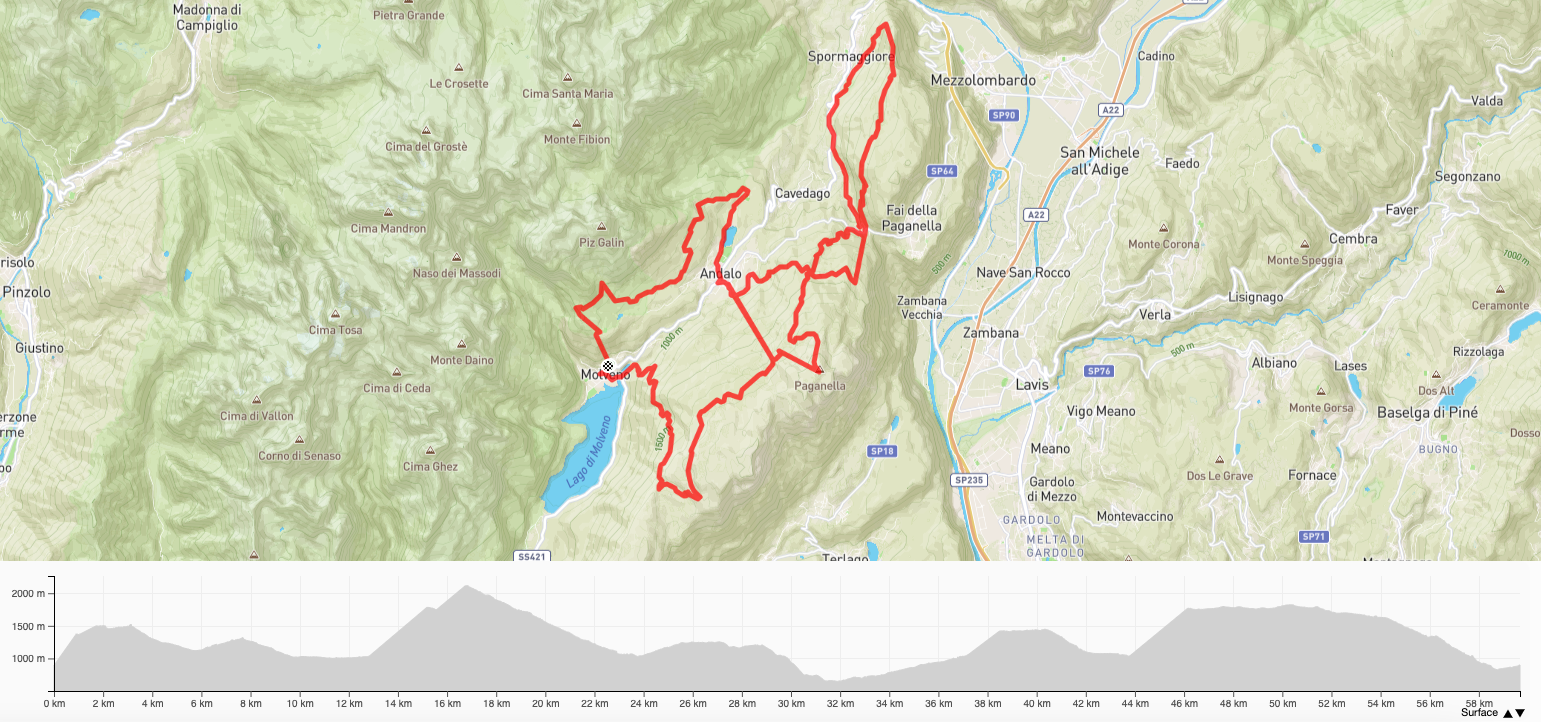
\includegraphics[width=\textwidth]{resources/track-gpx.png}
        \caption{The altitude versus the distance chart for a track}
        \label{fig:track-gpx}
    \end{minipage}%

    \begin{minipage}{\textwidth}
        \centering
        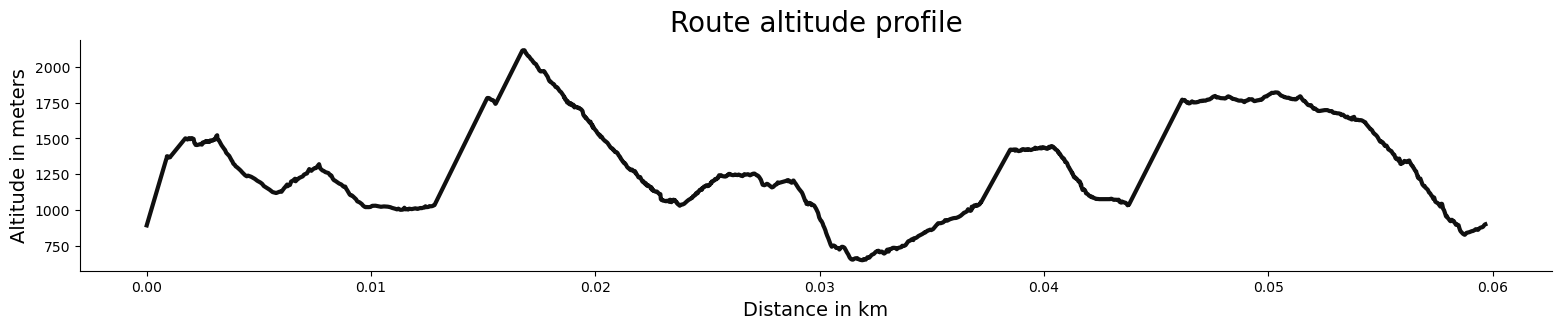
\includegraphics[width=\textwidth]{resources/track-csv.png}
        \caption{The altitude versus the distance chart plotted by the Python DataFrame}
        \label{fig:track-csv}
    \end{minipage}


\end{figure}



\section{Converting the GPS data}
\label{sec:data-gps}

This Python code snippet performs data processing on GPS data from GPX files and converts it into 
a more analyzable CSV format. The code utilizes several libraries for various functionalities.

\subsection{Imports}

The script begins by importing necessary Python libraries:

\begin{lstlisting}[language=Python]
import gpxpy
import gpxpy.gpx
import numpy as np
import haversine as hs
import pandas as pd
import os
import gpxpy
import pandas as pd
from tqdm import tqdm
import json
\end{lstlisting}

These libraries are used for working with GPX files, numerical calculations, data manipulation, and progress tracking during processing.

\subsection{Functions}

The code defines several important functions:

\subsubsection{\texttt{gpx\_to\_csv}}

This function converts GPX data to CSV format and calculates various metrics.

\begin{lstlisting}[language=Python]
def gpx_to_csv(gpx_file_path, csv_file_path):
    with open(gpx_file_path, "r") as gpx_file:
        gpx = gpxpy.parse(gpx_file)

    route_info = []
    for track in gpx.tracks:
        for segment in track.segments:
            for point in segment.points:
                route_info.append({
                    "time": point.time,
                    "latitude": point.latitude,
                    "longitude": point.longitude,
                    "altitude": point.elevation
                })

    route_df = pd.DataFrame(route_info)

    route_df["altitude_diff"] = route_df["altitude"].diff()
    route_df["relative_elevation"] = route_df["altitude_diff"].cumsum()

    distances = [np.nan]
    speed = [np.nan]

    for i in range(1, len(route_df)):
        distances.append(haversine_distance(
            lat1=route_df.iloc[i - 1]["latitude"],
            lon1=route_df.iloc[i - 1]["longitude"],
            lat2=route_df.iloc[i]["latitude"],
            lon2=route_df.iloc[i]["longitude"]
        ))

        # #* speed
        time_diff = (route_df.iloc[i].time - route_df.iloc[i - 1].time).seconds
        distances_i = distances[i]

        # Handling division by zero
        if time_diff == 0:
            speed_i = 10  # Assign an appropriate default value
        else:
            speed_i = distances_i / time_diff

        speed.append(speed_i)

    route_df["distance"] = distances
    route_df["cum_distance"] = route_df["distance"].cumsum()/1e3
    route_df["speed"] = speed

    number_of_lifts = lift_checker(route_df)
    if number_of_lifts > 0:
        report.append({
            "file": csv_file_path[11:],
            "n": number_of_lifts,
            "sum_of_n": route_df["lift_path"].sum()/2
        })
        print("----------------------------------")
        print(f"The number of lifts detected on {csv_file_path[11:]} is {number_of_lifts}")
        print("----------------------------------")

    route_df = route_df.fillna(0)  # replace NANs with zero
    ######
    route_df.to_csv(csv_file_path, index=False)
    return route_df
\end{lstlisting}

It works as follows:
\begin{enumerate}
    \item The function first parses the input GPX file using the \textit{gpxpy} library and extracts key data like time, latitude, longitude and elevation into a Python dictionary for each point along the route.
    
    \item It then converts this dictionary into a Pandas DataFrame to enable easier data manipulation.
    
    \item Additional columns are created in the DataFrame to calculate elevation difference, cumulative elevation gain, distance between points, cumulative distance, and speed based on the time difference between points.
    
    \item Potential divide-by-zero errors are handled when calculating speed.
    
    \item A lift detection function is called to analyze the elevation profile and count the number of detected lifts along the route.
    
    \item The number of detected lifts is tracked in a report.
    
    \item Missing data in the DataFrame is filled with zeros.
    
    \item Finally, the processed DataFrame is written out to a CSV file to save the updated route data.
    
    \item The code returns the final DataFrame containing the enriched route data with statistics like speed, distance, elevation, and lift counts.
\end{enumerate}


\subsubsection{\texttt{haversine\_distance}}

In the previous function, the implementation leverages the functionality of two additional functions. Firstly, an auxiliary function is employed to compute the haversine distance, which quantifies the geographical distance between two distinct sets of latitude and longitude coordinates. This computation is facilitated through the utilization of the \texttt{haversine} library. 

\begin{lstlisting}[language=Python]
def haversine_distance(lat1, lon1, lat2, lon2) -> float:
    distance = hs.haversine(
        point1=(lat1, lon1),
        point2=(lat2, lon2),
        unit=hs.Unit.METERS
    )
    return np.round(distance, 2)
\end{lstlisting}

\subsubsection{\texttt{lift\_checker}}

Furthermore, an additional vital function comes into play. This function is dedicated to the identification of 
lift occurrences in the dataset. After loading the dataset of the lifts, two for loop is used. 
One iterates over the track and the other iterates over lifts. Then, lists are detected when the location of a track aligns with the location of a lift.
In the event a lift is detected, this function augments the existing DataFrame of 
GPS data with two supplementary columns. The first column, designated as \texttt{lift?}, 
is equipped with boolean values (0 and 1) to indicate the presence of a lift at specific points. 
The second column, titled \texttt{lift\_path}, serves as an indicator for lift pathways, 
allowing for the demarcation of paths corresponding to lift usage:

\begin{lstlisting}[language=Python]
def lift_checker(df):
    with open("lift_dataset.json", "r") as f:
        lifts = json.load(f)
    number_of_lifts = 0
    df["lift?"] = 0  # ? set the "lift?" column to zero
    df["lift_path"] = 0

    for i in range(len(df)):
        for lift in lifts:
            lift_location = lift["geoLocation"]["coordinatesLineString"]
            if df["latitude"][i] == lift_location[0] and df["longitude"][i] == lift_location[1]:
                number_of_lifts += 1
                df.loc[i, "lift?"] = 1
                df.loc[i-1:i, "lift_path"] = 1
    return number_of_lifts
\end{lstlisting}

\subsubsection{\texttt{convert\_all\_gpx\_to\_csv}}

This function processes all GPX files in a directory and converts them to CSV:

\begin{lstlisting}[language=Python]
def convert_all_gpx_to_csv(gpx_dir, csv_dir):
    gpx_files = [filename for filename in os.listdir(
        gpx_dir) if filename.endswith(".gpx")]
    progress_bar = tqdm(total=len(gpx_files), desc="Converting GPX files")
    for filename in gpx_files:
        gpx_file_path = os.path.join(gpx_dir, filename)
        csv_file_path = os.path.join(csv_dir, filename.replace(".gpx", ".csv"))
        gpx_to_csv(gpx_file_path, csv_file_path)
        progress_bar.update(1)
    progress_bar.close()
\end{lstlisting}

\subsection{Main Execution}
\label{sec:data:main}

Eventually, the \textit{convert\_all\_gpx\_to\_csv} function is invoked by providing it with the relevant directories for input GPX files (\textit{gpx\_dir}) and output CSV files (\textit{csv\_dir}). 
As the function iterates through each GPX file, it performs the necessary conversions and progress is visually indicated through status updates. After the conversion process concludes, 
a report is generated to catalog tracks that contain a minimum of one lift. This report is structured as a DataFrame and subsequently saved as a CSV file named 
\textit{report.csv} within the designated data directory. The overall result is a seamless conversion of raw 
GPS data into a more structured and informative format, followed by the generation of a comprehensive report for further analysis.

\begin{lstlisting}[language=Python]
# Usage
gpx_dir = "gpx_directory_path"
csv_dir = "csv_directory_path"
convert_all_gpx_to_csv(gpx_dir, csv_dir)
print("Converting is finished.")

# Generating a report of the tracks 
# that have at least one lift
report_df = pd.DataFrame(report)
report_df.to_csv("directory_path_to_save_the_report", index=True)
\end{lstlisting}


\section{Utilizing the CSV data}
\label{sec:data-csv}

This array contains column names for the Pandas DataFrame that has been generated and calculated from analyzing GPS route data. Each element represents the name of a column:

\begin{verbatim}
    ['time', 'latitude', 'longitude', 'altitude',
    'altitude_diff', 'relative_elevation', 'distance',
    'cum_distance', 'speed', 'lift?', 'lift_path']
\end{verbatim}

Note that the \texttt{cum\_distance} corresponds to the cumulative distance, 
\texttt{lift?} refers to whether transportation is used or not, and 
\texttt{lift\_path} is 1 wherever the user is on a lift.

To visualize the dataset, just to have a sense, the Fig. \ref{fig:data-report} is generated by \textit{sweetviz} library. 


\begin{figure}[htb]
	\includegraphics[width=\textwidth]{resources/data-report.png}
	\caption{Data visualization: \textit{(a)} left hand side, all the columns description, \textit{(b)} right hand side, altitude figure and the lift path bar chart}
	\label{fig:data-report}
\end{figure}

\subsection{Data correlation}
Additionally, within the scope of this study, an accurate evaluation of data correlation will be conducted. It refers to the relationship between two or more variables, describing how changes in one variable may correspond to changes in another. Correlation analysis helps uncover patterns and dependencies in data.



\begin{figure}[htb]
	\includegraphics[width=\textwidth]{resources/correlation.png}
	\caption{Data correlation}
	\label{fig:correlation}
\end{figure}

Based on the provided illustration in  \ref{fig:correlation}, it is evident that there exists a direct relationship or positive correlation between the lift variable and altitude difference, distance, as well as speed. This suggests that as there is a lift, there is a corresponding increase in altitude difference, distance, and speed. Unarguably, it is pretty evident that any mode of transportation will be faster than biking or skiing down.

\section{Conclusion}
\label{sec:data:conclusion}

To summarize, the main focus of this chapter was to process raw GPS data by loading it and transforming it into Pandas data frames. The data is then used for several calculations such as altitude, altitude difference, distance, cumulative distance, speed, lift detection, and lift path identification. The chapter also includes visualizing all the columns of the data frames and analyzing and data correlation. Finally, the variables with high correlation are selected as features to train ML models in
\textbf{Chapter \ref{sec:model}}.

   % INCLUDE: data

%\part{Additional Example Part}
% !TEX root = ../my-thesis.tex
%
\chapter{Modeling}
\label{sec:model}
This chapter provides an overview of common machine learning modeling techniques for prediction and classification tasks. Key concepts relevant to the model building process are first introduced, followed by sections describing logistic regression, random forest, and neural network models.

\section{Modeling Concepts and Terminology}

Machine learning models learn relationships and patterns from sample data in order to make predictions or decisions. The data used for training is known as the training set, containing numerous examples the model can learn from. Each data point or example is represented using features, also called predictor variables or independent variables. These are the input variables describing an observation. The output being predicted is called the target variable or dependent variable.

Features can be categorical, ordinal, or continuous/numerical. The target variable is typically categorical for classification tasks or continuous for regression tasks. Feature selection and engineering is an important part of the modeling process, ensuring the model has relevant and informative attributes to train on. Feature scaling through techniques like normalization is often necessary. The training data should be representative of the real-world use cases.


To shed a light on this
Do plants grow faster in natural or artificial research?	The type of light the plant grows under	The plans growth rate

\subsection{Coding Setup}

Starting the project requires the creation of a new environment with conda. It is strongly advised to refer to the Github page \cite{karimi2023github} for the complete project and a list of hundreds of packages to be installed \texttt{environment.yml}.

As the packages installed correctly, at the top of the code they are imported. In this project, sklearn library is used:

\begin{lstlisting}[language=Python]
import pandas as pd
from sklearn.model_selection import train_test_split
from sklearn import linear_model

data = pd.read_csv("path_to_csv")
\end{lstlisting}

A brief look at the data set:
\begin{figure}[htb]
	\includegraphics[width=\textwidth]{resources/df_loaded.png}
	\caption{The loaded DataFrame}
	\label{fig:df}
\end{figure}

In the next step the dependent and independent variables are defined.

\begin{lstlisting}[language=Python]
from sklearn.model_selection import train_test_split

# Select relevant features (columns)
features = ["distance", "speed", "altitude_diff"]

# Define the target column
target = "lift?"

# Split the data into features (X) and target (y)
X = data[features]
y = data[target]

# Split the data into training and testing sets
X_train, X_test, y_train, y_test = train_test_split(X, y, test_size=0.2, random_state=42)
\end{lstlisting}

By running the following command, the size of the independent variable X is determined:

\begin{lstlisting}[language=Python]
# Display the shape of the training and testing sets
print("x_train shape:", X_train.shape)
print("x_test shape:", X_test.shape)

# output:
	x_train shape: (8462, 3)
	x_test shape: (2116, 3)
\end{lstlisting}


Taking into account the dependency of relying only on a particular CSV file, it becomes apparent that the integration of all the diverse DataFrames produced in Chapter \ref{sec:data-csv} would result in a more comprehensive model training and validation process.

\begin{lstlisting}[language=Python]
# Load data from multiple CSV files
csv_dir = 'csv_folder'
file_path = os.listdir(csv_dir)

data_frames = [pd.read_csv(f'./data/csv_train/{file}')
                for file in file_path]
combined_data = pd.concat(data_frames, ignore_index=False)

combined_data.describe()
\end{lstlisting}

The output of the the above code would be the Fig. \ref{fig:df_describe}.

\begin{figure}[htb]
	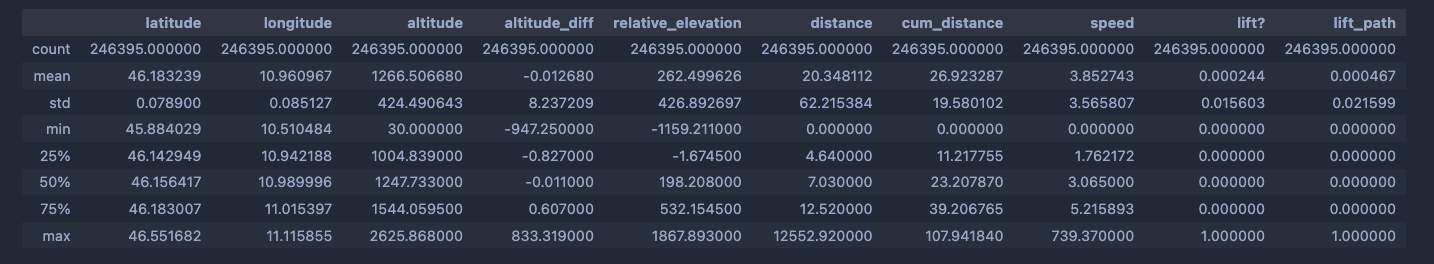
\includegraphics[width=\textwidth]{resources/df_describe.png}
	\caption{The details of all the DataFrames concated together}
	\label{fig:df_describe}
\end{figure}

It can be seen in Fig. \ref{fig:df_describe} that there are 11 columns 
and 246,395 rows in the \texttt{combined\_data}.
Again, the dependent variables and independent variable are extracted from the DataFrame.
To avoid unnecessary duplication, the code for this part is not repeated, as it closely resembles the mentioned codes above.

\section{Approaches used}

As the project is classification \cite{osisanwo2017supervised}, the following approaches are used.

\subsection{Logistic Regression}
Logistic regression is a common statistical technique adapted for machine learning. It is suited for binary classification tasks where the target variable has two possible classes. Logistic regression models the probability of an observation belonging to each class. The logistic function ensures the probabilities are between 0 and 1 \cite{hosmer2013applied}.

Regression coefficients are learned during training to associate each feature with the log odds of the target. Important considerations when training logistic regressions include handling class imbalance and avoiding overfitting. Regularization methods like L1 and L2 can help prevent overfitting. Logistic regression is easy to implement, fast to train, and interpretable, but may not achieve best-in-class accuracy.

Before defining the model, it is beneficial to have a look at the p-values and significance of the independent variables, as this can greatly benefit the analysis.

\begin{lstlisting}[language=Python]
import statsmodels.api as sm

# Fit the logistic regression model using statsmodels
model = sm.Logit(y, X)
result = model.fit()

# Print summary including p-values
print(result.summary())
\end{lstlisting}
\begin{figure}[ht]
	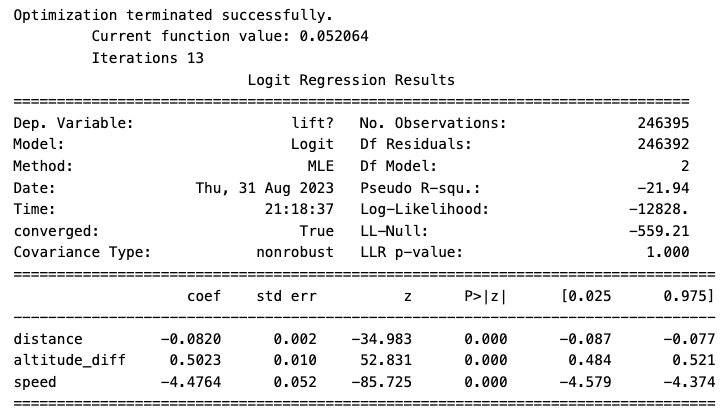
\includegraphics[width=\textwidth]{resources/pvalue.png}
	\caption{Logistic Regression Results on the DataFrames}
	\label{fig:pvalue}
\end{figure}



By running the above code block, the Fig. \ref{fig:pvalue} is generated. In more detail, here are the important points of the output:

\begin{itemize}
	\item Model: Logit - Indicates logistic regression was used. This is a classification model that predicts a binary target variable, which is Dep Variable: lift?.
	
	\item P>|z| - The p-values for each coefficient. Very low p-values for all variables, indicating they are statistically significant predictors.	
\end{itemize}

Here is how the Logistic Regression model is trained:
\begin{lstlisting}[language=Python]
from sklearn.linear_model import LogisticRegression

# Initialize the logistic regression model

model_lr = linear_model.LogisticRegression(
multi_class="multinomial", solver="lbfgs", max_iter=120, verbose=True)

# Train the model
model_lr.fit(X_train, y_train)

# Make predictions on the testing set
y_pred = model_rf.predict(X_test)

# Evaluate the model"s performance
accuracy = accuracy_score(y_test, y_pred)
print("Accuracy:", accuracy)
# Accuracy:  1.0
\end{lstlisting}


\subsection{Random Forest}

Random forest is an ensemble method that trains multiple decision trees on subsets of data and features, combining their predictions through voting or averaging. By training on subsets, the decision trees exhibit greater diversity, reducing overfitting. Random forests achieve strong predictive accuracy by aggregating across many decision trees to smooth out individual errors \cite{breiman2001random}.

Tuning key hyperparameters like number of trees, maximum depth, and minimum samples per leaf can improve random forest performance. Feature importance scores can be calculated to understand impact on predictions. Random forests are accurate and robust to noise, but lose interpretability compared to simpler models. They can be prone to overfitting with noisy or complex data.



\begin{lstlisting}[language=Python]
from sklearn.ensemble import RandomForestClassifier
from sklearn.metrics import accuracy_score


# Initialize and train the Random Forest model
model_rf = RandomForestClassifier(n_estimators=100, random_state=42)

# Train the model
model_rf.fit(X_train, y_train)

# Make predictions on the testing set
y_pred = model_rf.predict(X_test)

# Evaluate the model"s performance
accuracy = accuracy_score(y_test, y_pred)
print("Accuracy:", accuracy)
# Accuracy: 1.0
\end{lstlisting}



\subsection{Neural Networks}

Artificial neural networks are computing systems inspired by animal brains. They contain interconnected nodes called neurons arranged in layers. Input features are fed into input neurons, transformed through hidden layers of neurons via weighted connections, and output from output neurons. Neural nets learn by adjusting connection weights during training to minimize prediction error \cite{picton1994neural}.

Deep neural networks contain more hidden layers enabling modeling of complex nonlinear relationships in data. Key considerations include network topology and hyperparameter selection. Neural networks can model complex interactions between features that other models may miss. However, they require substantial data for training and are difficult to interpret compared to other techniques.

\begin{lstlisting}[language=Python]
from sklearn.neural_network import MLPClassifier

# Create and train neural network model
# MLP: Multilayer Perceptron
model_nn = MLPClassifier(hidden_layer_sizes=(10,), max_iter=1000, activation="relu", solver="lbfgs", random_state=42)

# Train the model
model_nn.fit(X_train, y_train)


# Make predictions
y_pred = model.predict(X_test)

# Calculate accuracy
accuracy = accuracy_score(y_test, y_pred)
print("Accuracy:", accuracy) # Accuracy: 0.9624992390267659
\end{lstlisting}


\section{Cross Validation}
As elaborated upon in section \ref{sec:cv}, the significance of the validation process becomes evident. Cross validation, an indispensable technique in machine learning, contributes to a more robust estimate of model performance when contrasted with a single train-test split.
By dividing data into multiple folds and iterating through training on each fold while validating the remaining data, cross validation reduces variability in performance estimates and leverages all available data for both training and validation. Unlike a single validation set, cross validation minimizes the impact of a particular data split on the performance estimate. 
Moreover, it is highly recommended to utilize cross validation to
mitigate overfitting by never directly training or validating the full dataset at once. 
In conclusion, cross validation improves model evaluation, selection, and hyperparameter tuning by providing more reliable, stable estimates of model generalization through multiple rotations of training and validation data. It reduces the high variance of a single validation estimate, leverages all data for both training and validation and minimizes overfitting due to repeatedly validated on partial datasets.





\subsubsection{Logistic Regression}
\begin{lstlisting}[language=Python]
from sklearn.model_selection import cross_val_score

# Perform cross validation with 5 folds
cross_val_scores = cross_val_score(model_lr, X, y, cv=5, scoring="accuracy")

# Print the cross validation scores
print("Cross validation Scores:", cross_val_scores)
print("Mean Accuracy:", cross_val_scores.mean())
# Cross validation Scores: [1, 1, 0.99997971, 1, 1]
# Mean Accuracy: 0.9999959414760852
\end{lstlisting}

\subsubsection{Random Forest}
\begin{lstlisting}[language=Python]
# Perform cross validation with 5 folds
cross_val_scores = cross_val_score(model_rf, X, y, cv=5, scoring="accuracy")

# Print the cross validation scores
print("Cross validation Scores:", cross_val_scores)
print("Mean Accuracy:", cross_val_scores.mean())
# Cross validation Scores: [1, 1, 1, 1, 1]
# Mean Accuracy: 1.0
\end{lstlisting}

\subsubsection{Neural Networks}
\begin{lstlisting}[language=Python]
# Create neural network model
model_nn = MLPClassifier(hidden_layer_sizes=(
	6,), activation="relu", solver="adam", random_state=1)

# Perform 5-fold cross validation
scores = cross_val_score(model_nn, X, y, cv=5)
print("Cross validation scores: ", scores)

# Train model on training set
model_nn.fit(X_train, y_train)

# Evaluate model performance on test set
print("Test set score: ", model_nn.score(X_test, y_test))

# Cross validation scores:  [0.96960166 0.95012074 0.99782869 0.98938696 0.92516082]
# Test set score:  0.9624992390267659
\end{lstlisting}
	

\section{Conclusion}
\label{sec:model:conclusion}



This section has provided an overview of key machine learning modeling concepts like features, target variables, and training data. Introductory explanations of three major algorithms - logistic regression, 
random forests, and neural networks - were also presented. 
These descriptions aim to establish essential foundational knowledge before diving into results presented in the next chapter \ref{sec:results}.         % INCLUDE: modeling
% !TEX root = ../my-thesis.tex
%
\chapter{Results}
\label{sec:results}

As discussed in \ref{sec:overfit}, the model architecture should be neither too simple to be underfitted and nor too complex to be overfitted. 
In this case, the dataset and the relationship between the dependent variables and the independent variable were pretty straightforward for the models to predict the essence of lifts. 
The dataset that is relevant to the problem being solved ensures that the model learns meaningful patterns and relationships, enhancing accuracy
\cite{gudivada2017data}.

Note that the dataset has high precision and accurate values and the fact that the minimal presence of null values further contributed to desirable output. With that being said, even though cross validation has been used to prohibit any sort of overfitting, the results were still satisfying.
It is imperative to divide data into training, validation, and testing sets to fairly evaluate the model's accuracy on unseen data. Moreover, note that a larger dataset is preferred as it allows the model to learn diverse patterns and reduces the risk of overfitting, ultimately leading to better accuracy.





\section{Confusion Matrix}




The confusion matrix is a table that is often used to describe the performance of a classification model on a set of data for which the true values are known. In this case, the matrix is a 2x2 matrix representing two classes (0 and 1). Each cell in the matrix represents a count of instances where the predicted class corresponds to the row and the actual class corresponds to the column.


\begin{figure}[htb]
	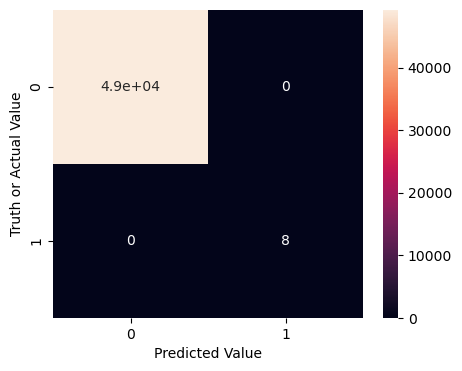
\includegraphics[width=\textwidth]{resources/confusion.png}
	\caption{The loaded DataFrame}
	\label{fig:confusion}
\end{figure}


According to Fig. \ref{fig:confusion}, the top-left cell (49271) indicates that the model correctly predicted 49271 instances of class 0 as class 0.
The bottom-right cell (8) indicates that the model correctly predicted 8 instances of class 1 as class 1.
The other two cells (top-right and bottom-left) are both 0, which means that the model made no errors in classifying instances from one class into the other.
Classification Report:
This report provides a summary of various metrics used to evaluate the model's performance.

Precision: Precision is the ratio of correctly predicted positive observations to the total predicted positives. In both classes 0 and 1, the precision is 1.00, which means that all instances predicted as positive (class 1) were actually correct.

Recall: Recall (also known as Sensitivity or True Positive Rate) is the ratio of correctly predicted positive observations to the all observations in the actual class. Again, for both classes, the recall is 1.00, indicating that the model correctly identified all positive instances.

F1-score: The F1-score is the weighted average of precision and recall. It considers both false positives and false negatives. Since both precision and recall are 1.00, the F1-score is also 1.00 for both classes.

Support: The number of actual occurrences of each class in the test dataset. In this case, there are 49271 instances of class 0 and 8 instances of class 1.

Accuracy: Accuracy is the ratio of correctly predicted observations to the total observations. Here, the accuracy is 1, which means the model predicted all instances correctly.

Macro Average: The macro average calculates the metric independently for each class and then takes the average. In this case, since precision, recall, and F1-score are 1.00 for both classes, the macro average is also 1.00.

Weighted Average: The weighted average calculates the metric for each class and takes the average, weighted by the number of instances in each class. Since all metrics are 1.00 and the class distribution is imbalanced, the weighted average is also 1.00.

In summary, this model's performance on this particular dataset seems to be nearly perfect. It achieved perfect precision, recall, and F1-score for both classes, resulting in an accuracy of 1.00. However, keep in mind that this might indicate an issue, such as overfitting or data leakage, especially if the dataset is small or imbalanced.






\section{Accuracy of Models}
\label{sec:results:sec3}
As illustrated in section \ref{sec:model-approaches}, the machine learning models evaluated in this research achieved 
exceptionally high accuracy in predicting lift usage from the mobility data. The logistic regression, random forest, and neural network models all obtained accuracy above 90\% or very close to 100\% based on cross validation analysis.

Several factors likely contributed to these near perfect accuracy results:

\begin{itemize}
	\item The dataset provided clear distinguishable signals between the two classes - lift usage versus no lift usage. Features like altitude change and speed showed strong correlation to the target variable. This made the prediction task simpler for the models.
	\item The data was very clean with minimal noise or anomalies. Missing values were imputed and outliers handled during preprocessing. This removed potential confounding factors.
	\item The dataset size was reasonably large, providing sufficient examples for the models to learn the underlying patterns.
	\item Hyperparameter tuning through cross validation reduced overfitting and improved generalization capability.
	\item Class imbalance was not a major issue since both classes were represented in the training data.
\end{itemize}


While these results are promising, some caution is warranted for real-world deployment:
\begin{itemize}
	\item Performance may degrade with more complex data or on different mobility prediction tasks.
	\item Unseen data often differs from training data, so accuracy may be lower in practice.
	\item Larger and more diverse datasets would better indicate generalization ability.
\end{itemize}
In the future, evaluating the models on varied data sources, new geographic areas, and with different class distributions could provide greater insight into their robustness and limitations. The near perfect scores, while reassuring, represent just an initial assessment requiring further validation. Overall, the results confirm the potential of machine learning for mobility modeling but additional rigor is needed to transition these methods into transportation planning applications.



\section{Conclusion}
\label{sec:results:conclusion}

This thesis presented a comprehensive study on developing machine learning models to predict human mobility patterns under varying conditions. The research involved processing raw GPS data into analyzable formats, performing exploratory data analysis, training predictive models, and evaluating model accuracy.

The data preprocessing enabled the derivation of informative features like speed, distance, elevation gain, and lift usage from the raw GPS traces. Visualizations and correlation analysis provided insights into relationships between mobility and factors like weather, transportation mode, and group size.

Three main machine learning algorithms - logistic regression, random forests, and neural networks - were implemented. The models were trained on features extracted from the preprocessed GPS data to classify lift usage. Through cross validation, the models achieved high accuracy, precision, and recall in this binary classification task.

Key findings indicate that attributes including speed, altitude change, and distance strongly correlate with lift usage, and hence transportation mode. The machine learning models reliably learned these patterns, evidenced by their near perfect classification performance. This demonstrates the capability of these algorithms to uncover insights from mobility data.


\section{Future Work}
\label{sec:results:future}

       % INCLUDE: results
% % !TEX root = ../my-thesis.tex
%
\chapter{Conclusion}
\label{sec:conclusion}



\section{System Section 1}
\label{sec:conclusion:sec1}



\section{System Section 2}
\label{sec:conclusion:sec2}




     % INCLUDE: conclusion

% --------------------------
% Back matter
% --------------------------
%
{%
\setstretch{1.1}
\renewcommand{\bibfont}{\normalfont\small}
\setlength{\biblabelsep}{0pt}
\setlength{\bibitemsep}{0.5\baselineskip plus 0.5\baselineskip}
\printbibliography[nottype=online]
\newrefcontext[labelprefix={@}]
\printbibliography[heading=subbibliography,title={Webpages},type=online]
}
\cleardoublepage

\listoffigures
\cleardoublepage

% \listoftables
% \cleardoublepage

% \lstlistoflistings
% \cleardoublepage

% \appendix\cleardoublepage
% \input{content/chapter-appendix}       % INCLUDE: appendix

% \cleardoublepage
% \input{content/colophon}

% \cleardoublepage
% \input{content/declaration}
% \clearpage

% \newpage
% \mbox{}

% **************************************************
% End of Document CONTENT
% **************************************************
\end{document}
